\section{Ablaufbeschreibung}
\label{sec:ablaufbeschreibung}

Im folgenden sind Ablaufbeschreibungen für die Anwendungsfälle Browserstart,
Eruieren der Ausführung und Suchanfrage zu finden. Die übrigen Anwendungsfälle
werden im Rahmen dieser Modularbeit nicht genauer erfasst. 

Die Diagramme sind als Aktivitätsdiagramme - wie auch alle weiteren Diagramme in
diesem Dokument - nach der \acs{UML} verfasst\footnote[1]{Die \acs{UML} wurde
als geeignete Modellierungssprache ausgewählt, da sie relativ verbreitet ist,
einen einheitlichen Standard für eine grosse Anzahl von Diagrammtypen bietet und
weil viel Literatur dazu gefunden werden kann, was das erarbeiten der Syntax und
Semantik auch für Leute ohne grosse Vorkentnisse stark erleichtert.}.

\subsection{Browserstart}

In Abbildung \ref{fig:ablauf-start} ist der Ablauf für den Anwendungsfall
\enquote{Browserstart} in Bezug auf den für \textit{Google Muddle} relevanten
Teil genauer beschrieben.
\\[\intextsep]
\begin{minipage}{\linewidth}
\centering%
\includegraphics[scale=0.4,clip=]{img/ablauf-start.eps}%
\figcaption{Ablaufbeschreibung Browserstart}%
\label{fig:ablauf-start}%
\end{minipage}

\newpage

\subsection{Eruieren der Ausführung}

Abbildung \ref{fig:ablauf-ausfuehrung} zeigt die Ablaufbeschreibung für den
Anwendungsfall \enquote{Eruieren der Ausführung}.
\\[\intextsep]
\begin{minipage}{\linewidth}
\centering%
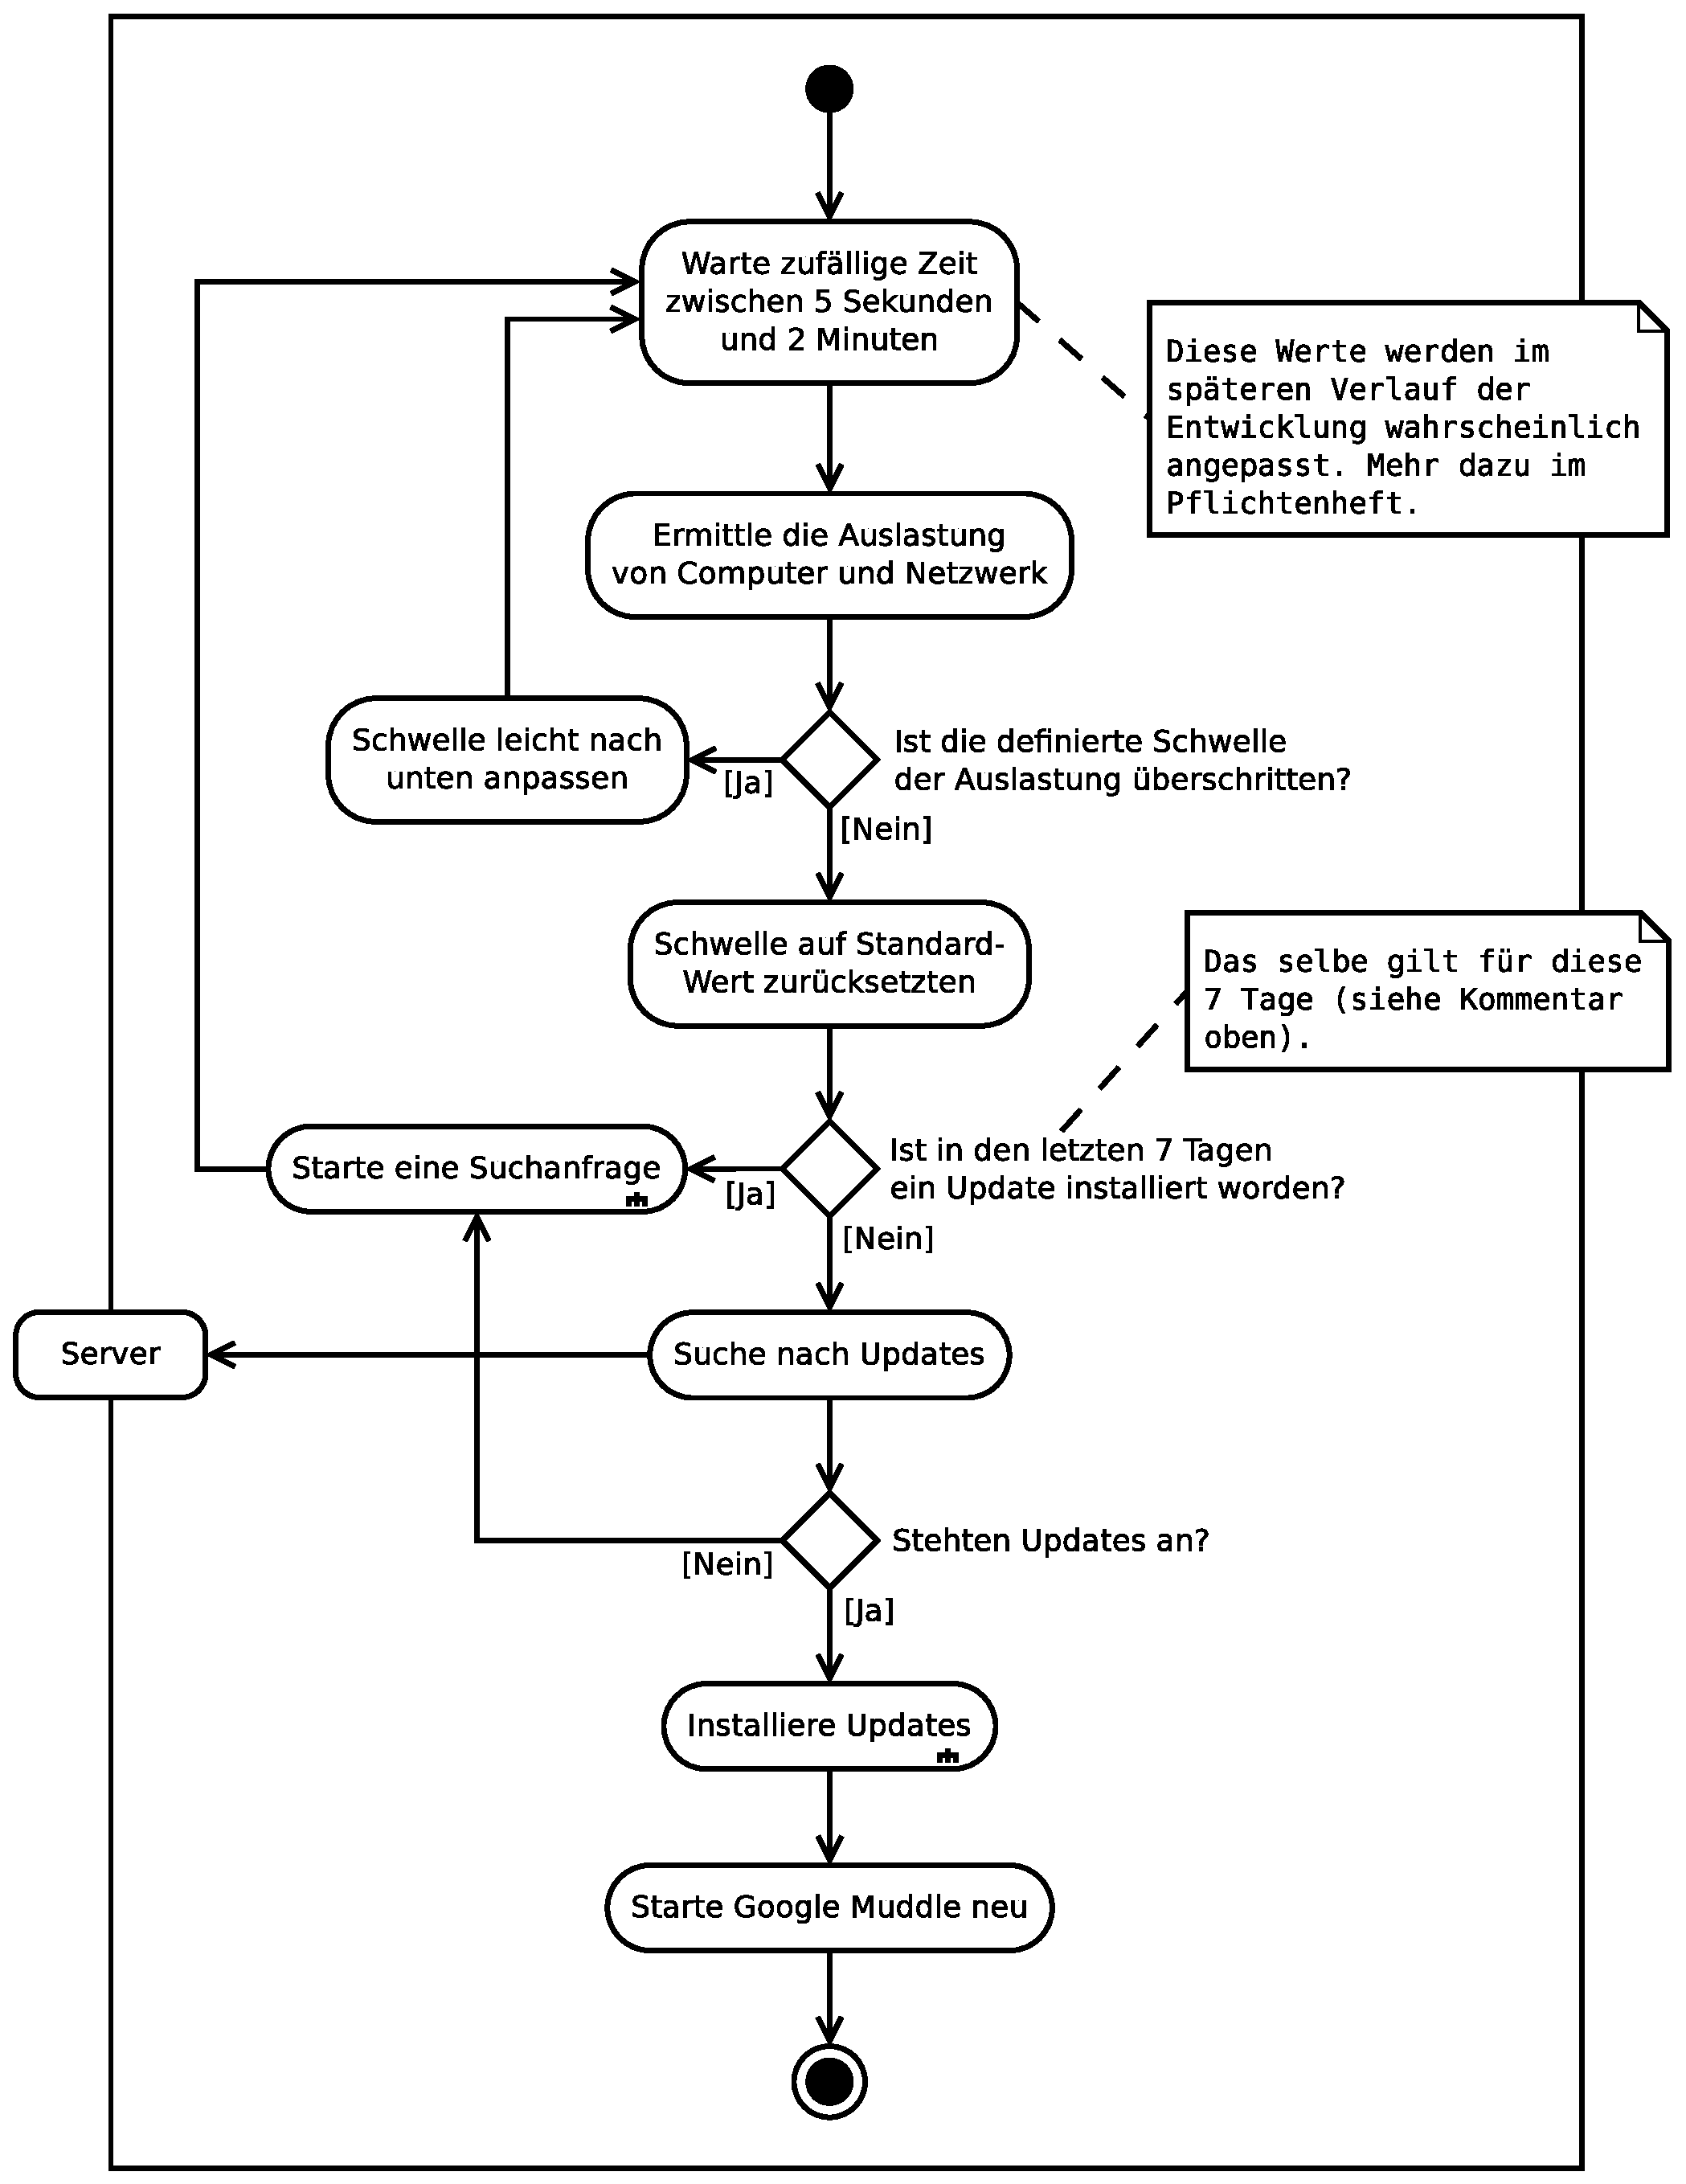
\includegraphics[scale=0.4,clip=]{img/ablauf-ausfuehrung.eps}%
\figcaption{Ablaufbeschreibung Eruieren der Ausführung}%
\label{fig:ablauf-ausfuehrung}%
\end{minipage}

\newpage

\subsection{Suchanfrage}

In Abbildung \ref{fig:ablauf-suche} wird die Ablaufbeschreibung für den
Anwendungsfall \enquote{Suchanfrage} dargestellt.
\\[\intextsep]
\begin{minipage}{\linewidth}
\centering%
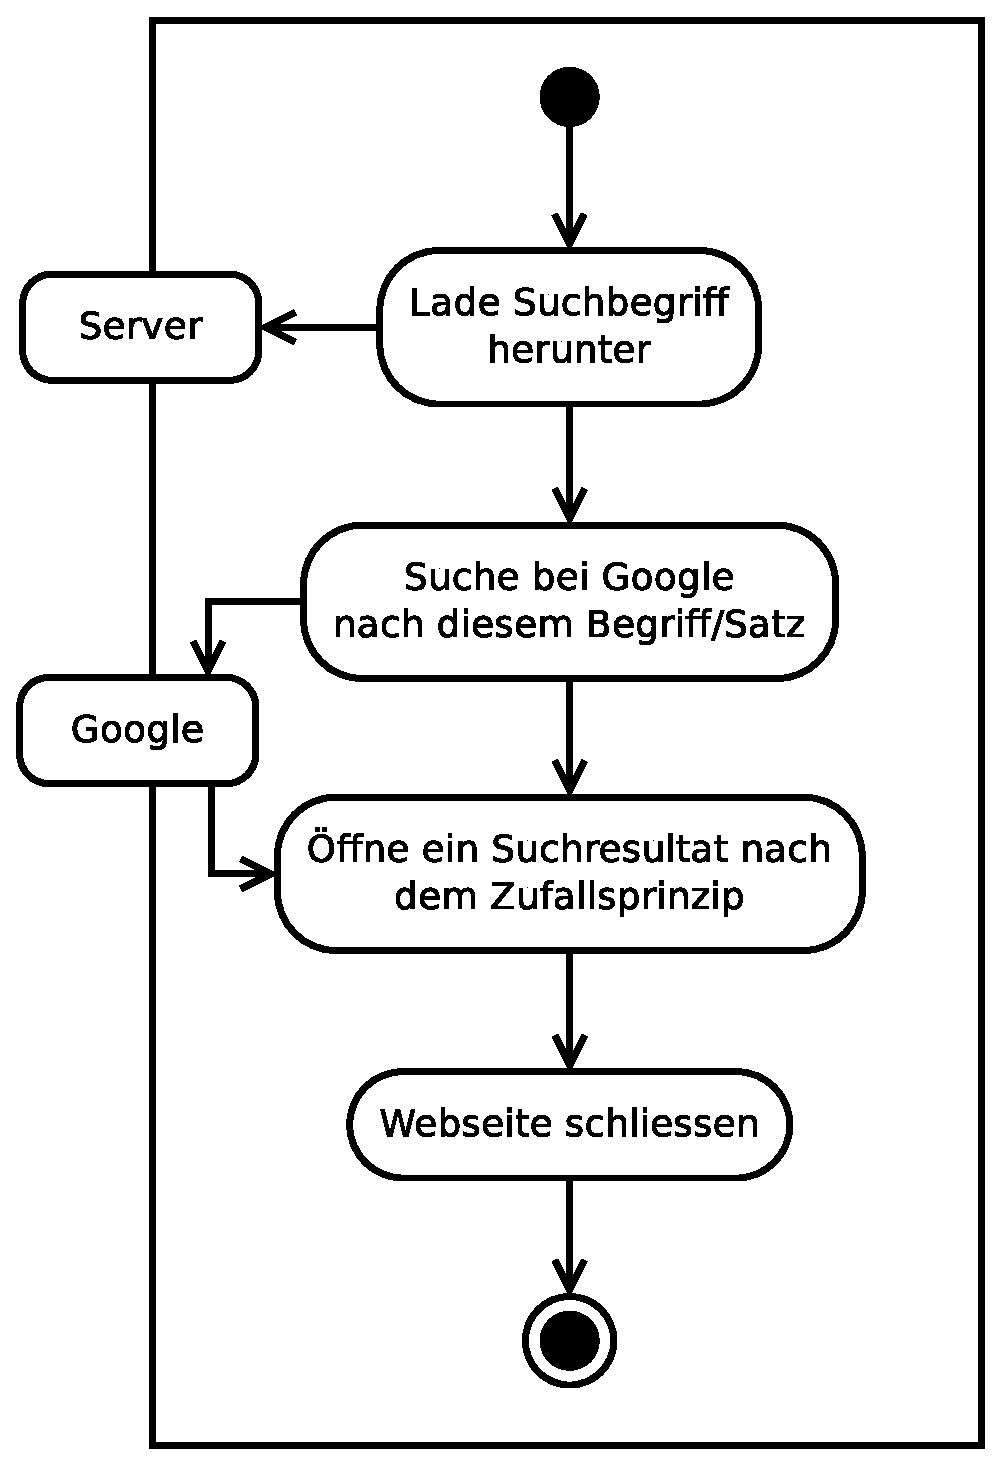
\includegraphics[scale=0.4,clip=]{img/ablauf-suche.eps}%
\figcaption{Ablaufbeschreibung Suchanfrage}%
\label{fig:ablauf-suche}%
\end{minipage}

\newpage

\subsection{Datenrücksendung}

Diese Ablaufbeschreibung wird im Rahmen der Modularbeit nicht erfasst.

\subsection{Update}

Diese Ablaufbeschreibung wird im Rahmen der Modularbeit nicht erfasst.

\subsection{Browserende}

Diese Ablaufbeschreibung wird im Rahmen der Modularbeit nicht erfasst.

